\section{Giới thiệu}\label{sec:intro}
\frame{\tableofcontents[currentsection]}
\begin{frame}{Giới thiệu}

\begin{itemize}
    \item <1-> Là một nhánh của bài toán tái định danh.
    \item <2-> Dựa vào các thuộc tính đã biết trước (\textit{tuổi tác, ngoại hình, giới tính, ...}) để nhận diện lại đối tượng.
\begin{figure}[H]
    \centering
    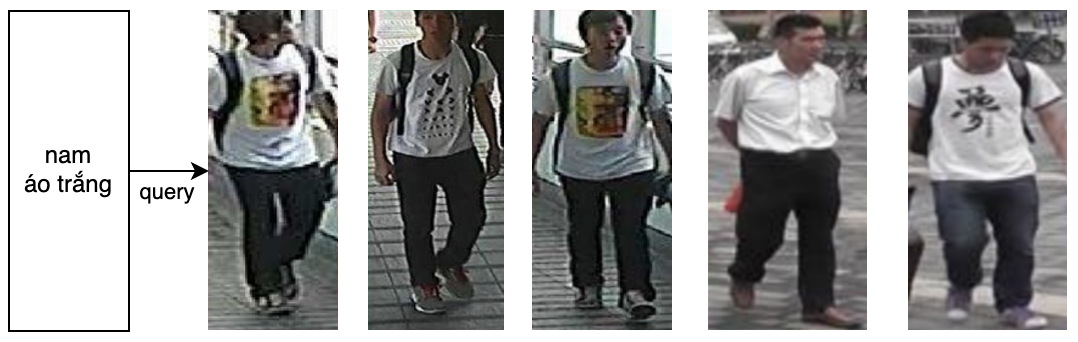
\includegraphics[width=13cm]{images/example.png}
    % \caption{Ví dụ về truy tìm đối tượng}
    \label{fig:example}
\end{figure}
\end{itemize}
\end{frame}
